\section{Entrega parcial 1}

\subsection{Realizar un análisis de los datos a utilizar y principales funcionalidades a  implementar que dan sentido a la realización del proyecto}

La problemática a abordar en este proyecto es la necesidad que tienen los colegios de llevar un registro de asistencia de sus estudiantes para cada año escolar, y para ello, la principal información que deberemos manejar son los \textbf{estudiantes} y los \textbf{cursos}. Los cursos se dividirán en diferentes niveles y cada nivel subdividirá en paralelos, cada uno de estos contará con la información del profesor a cargo de este curso y la lista de alumnos correspondiente.\\

Los alumnos contarán con información básica de ellos (nombre, rut, apellido, etc.) y cada uno contará con su registro de asistencia correspondiente al año escolar, con esto buscamos que se generen archivos que muestren la lista de estudiantes de cada curso y la asistencia de estos.\\

\textbf{Funcionalidades principales:}
\begin{itemize}
    \item Registrar asistencia de un curso para cada dia de clases.
    \item Registrar inasistencias.
    \item Registro de salidas antes de horario.
    \item Consultar registro de asistencia, inasistencias y  salidas antes de horario de cualquier día del año.
\end{itemize}

\textbf{Funcionalidades secundarias:}
\begin{itemize}
    \item Calcular porcentaje de asistencia
    \item Generar ranking de asistencia en distintos niveles del colegio
    \item Generar reportes en base a la asistencia
\end{itemize}

\textbf{Entidades:}
\begin{itemize}
    \item Alumnos del colegio
    \item Cursos y niveles
    \item Profesores
    \item Apoderados
    \item Registro de asistencia
\end{itemize}
	
\textbf{Manejo de datos:}
\begin{itemize}
    \item El software desarrollado tiene la capacidad de conectarse tanto a una base de datos MySQL (o MariaDB), y también de trabajar con datos almacenados de forma local a través de un archivo CSV, desarrollando con ello todas las funcionalidades necesarias para leer, insertar, actualizar o eliminar datos desde cualquiera sea el origen de datos.\\
    Para trabajar con la base de datos, el software incorpora las configuraciones necesarias para ejecutar, a través de \textbf{docker}, una base de datos en MySQL con los datos iniciales, y se conecta a ella de forma predeterminada, utilizando las credenciales incorporadas en el archivo \textbf{.env}, que por razones de seguridad, no está incluído en el repositorio de GitHub, pero sí en la entrega final.
    \item Para efecto de trabajar con datos iniciales, se creó una clase Fakedata que incluye una librería externa (Faker). Esta clase permite crear datos iniciales aleatorios, y los guarda en los ficheros CSV respectivos, utilizando la clase Datafile de manejo de archivos.
\end{itemize}

\clearpage

\subsection{Diseño conceptual de clases del Dominio y su código en Java}

\begin{figure}[h]
    \centering
    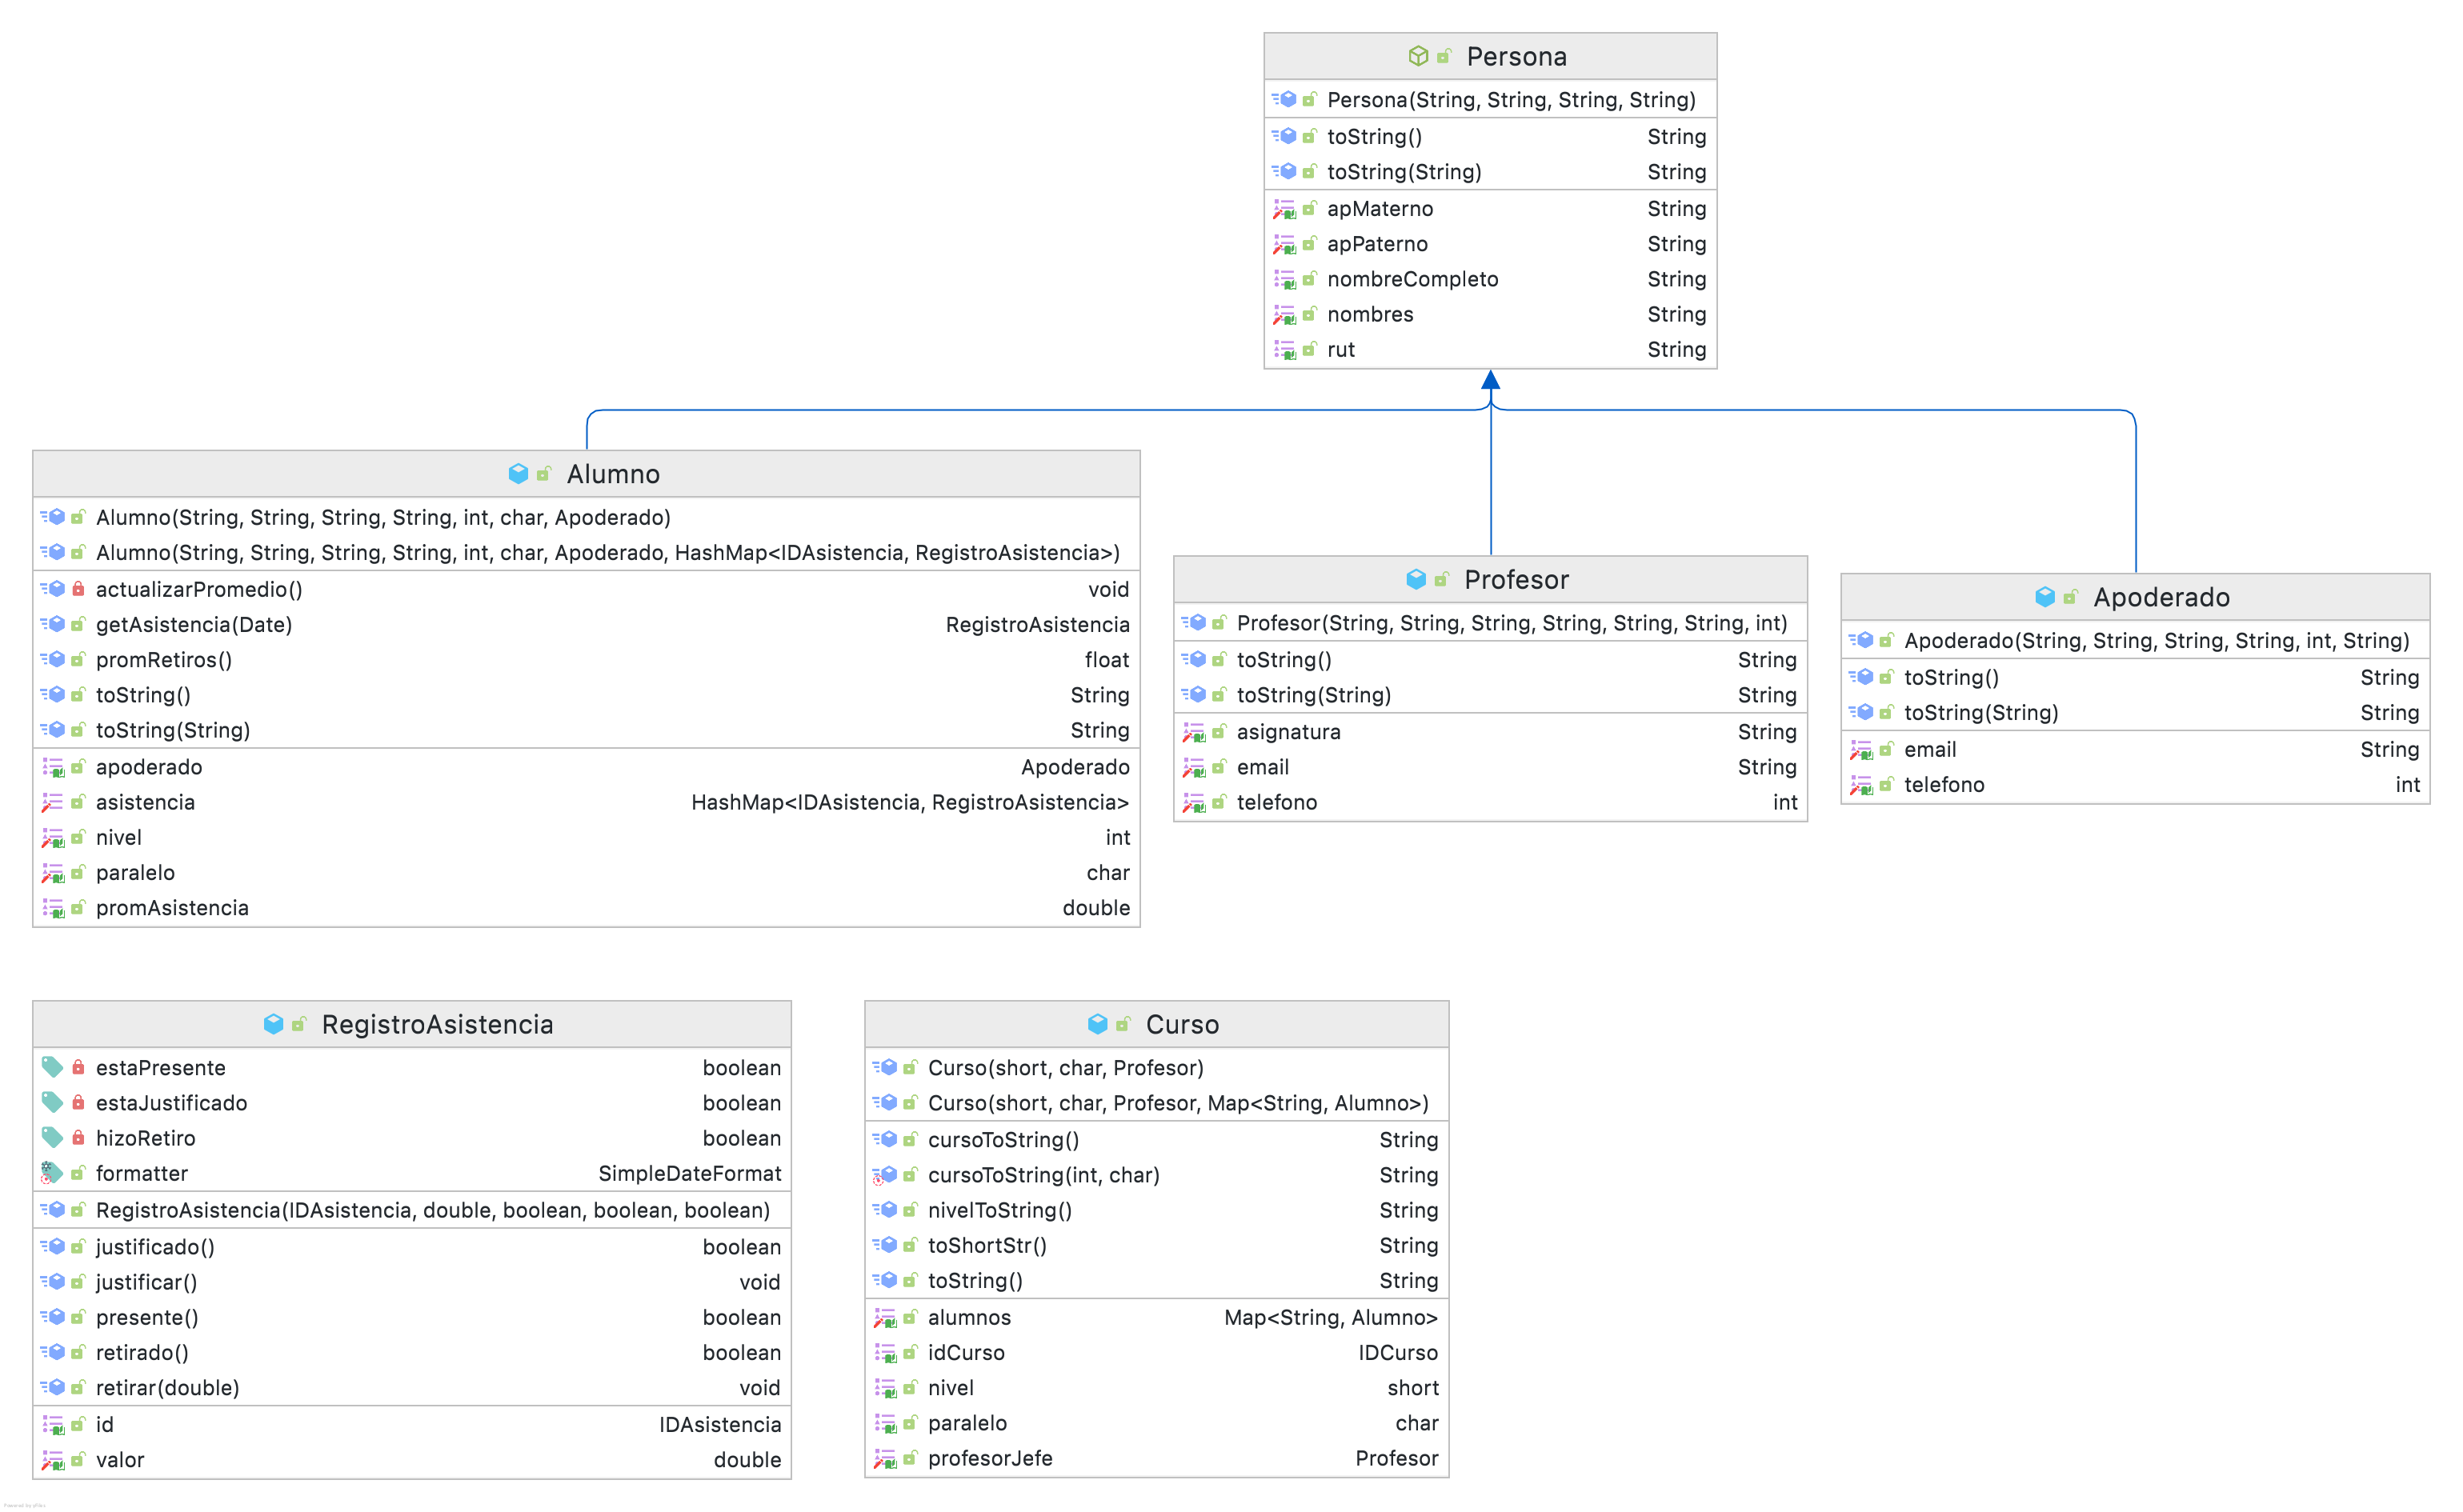
\includegraphics[width=0.9\textwidth]{contents/img/img1}
    \caption{Clases del dominio}
    \label{fig:img1}
\end{figure}

La clase \textbf{Persona} contendrá los datos genéricos de una persona, y será la clase padre de \textbf{Apoderado}, \textbf{Alumno} y \textbf{Profesor}. Además está la clase \textbf{Curso} que posee el nivel, valor numérico de 1 a 12, una letra identificadora de paralelo, un profesor jefe, y un Hashmap de alumnos, cuya llave será el RUT del alumno correspondiente.\\

En el caso de \textbf{Apoderado}, este hereda de \textbf{Persona} y además tiene los datos de contacto del apoderado de cada alumno. \textbf{Alumno} contiene a su apoderado, y lleva su registro de asistencia correspondiente al año escolar.\\
	
Para el manejo de los datos, se utilizarán \textbf{interfaces} que nos permitan estandarizar la forma de obtener y manejar los datos, para poder incorporar en el futuro, de una forma más simple, manejo de bases de datos.\\

\begin{figure}[h]
    \centering
    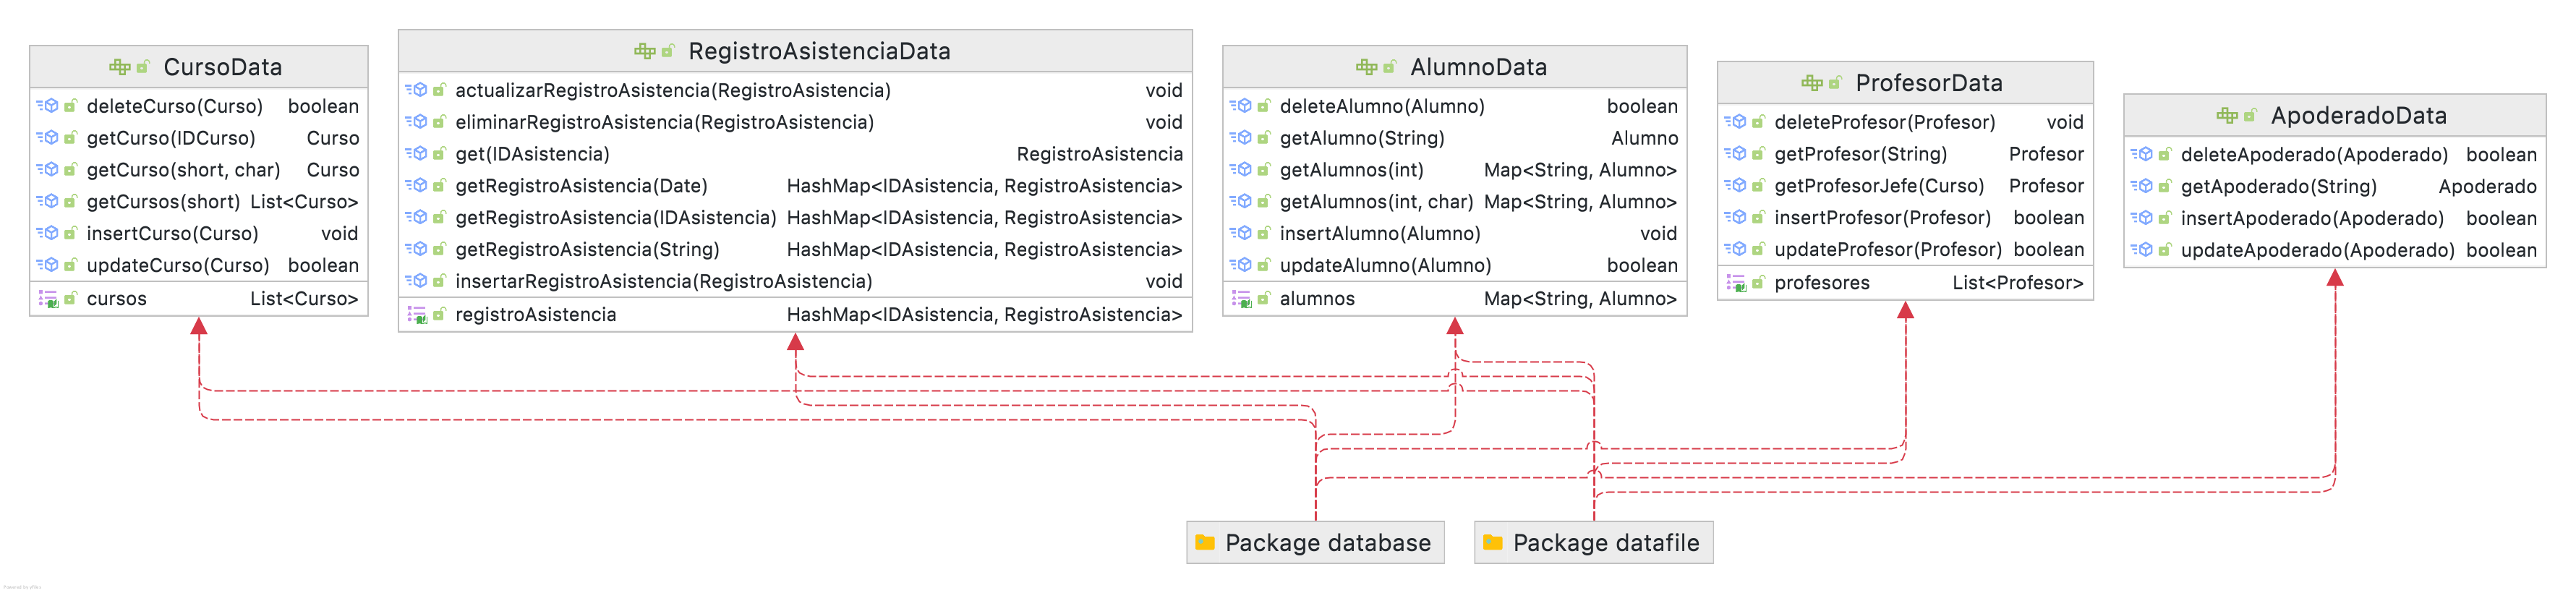
\includegraphics[width=0.9\textwidth]{contents/img/img2}
    \caption{Clases para manejo de datos}
    \label{fig:img2}
\end{figure}

Para el manejo de los archivos de texto en donde se almacenan los datos, se utilizará una clase dedicada a trabajar con ellos. Esta clase contendrá los métodos que posibilitan la inserción, listado, eliminación y actualización de los datos, entregados como texto CSV, separado por punto y coma (;). Para llevar los datos al formato CSV, la clase contiene un método estático que permite transformar una lista de String al texto CSV.

\begin{figure}[h]
    \centering
    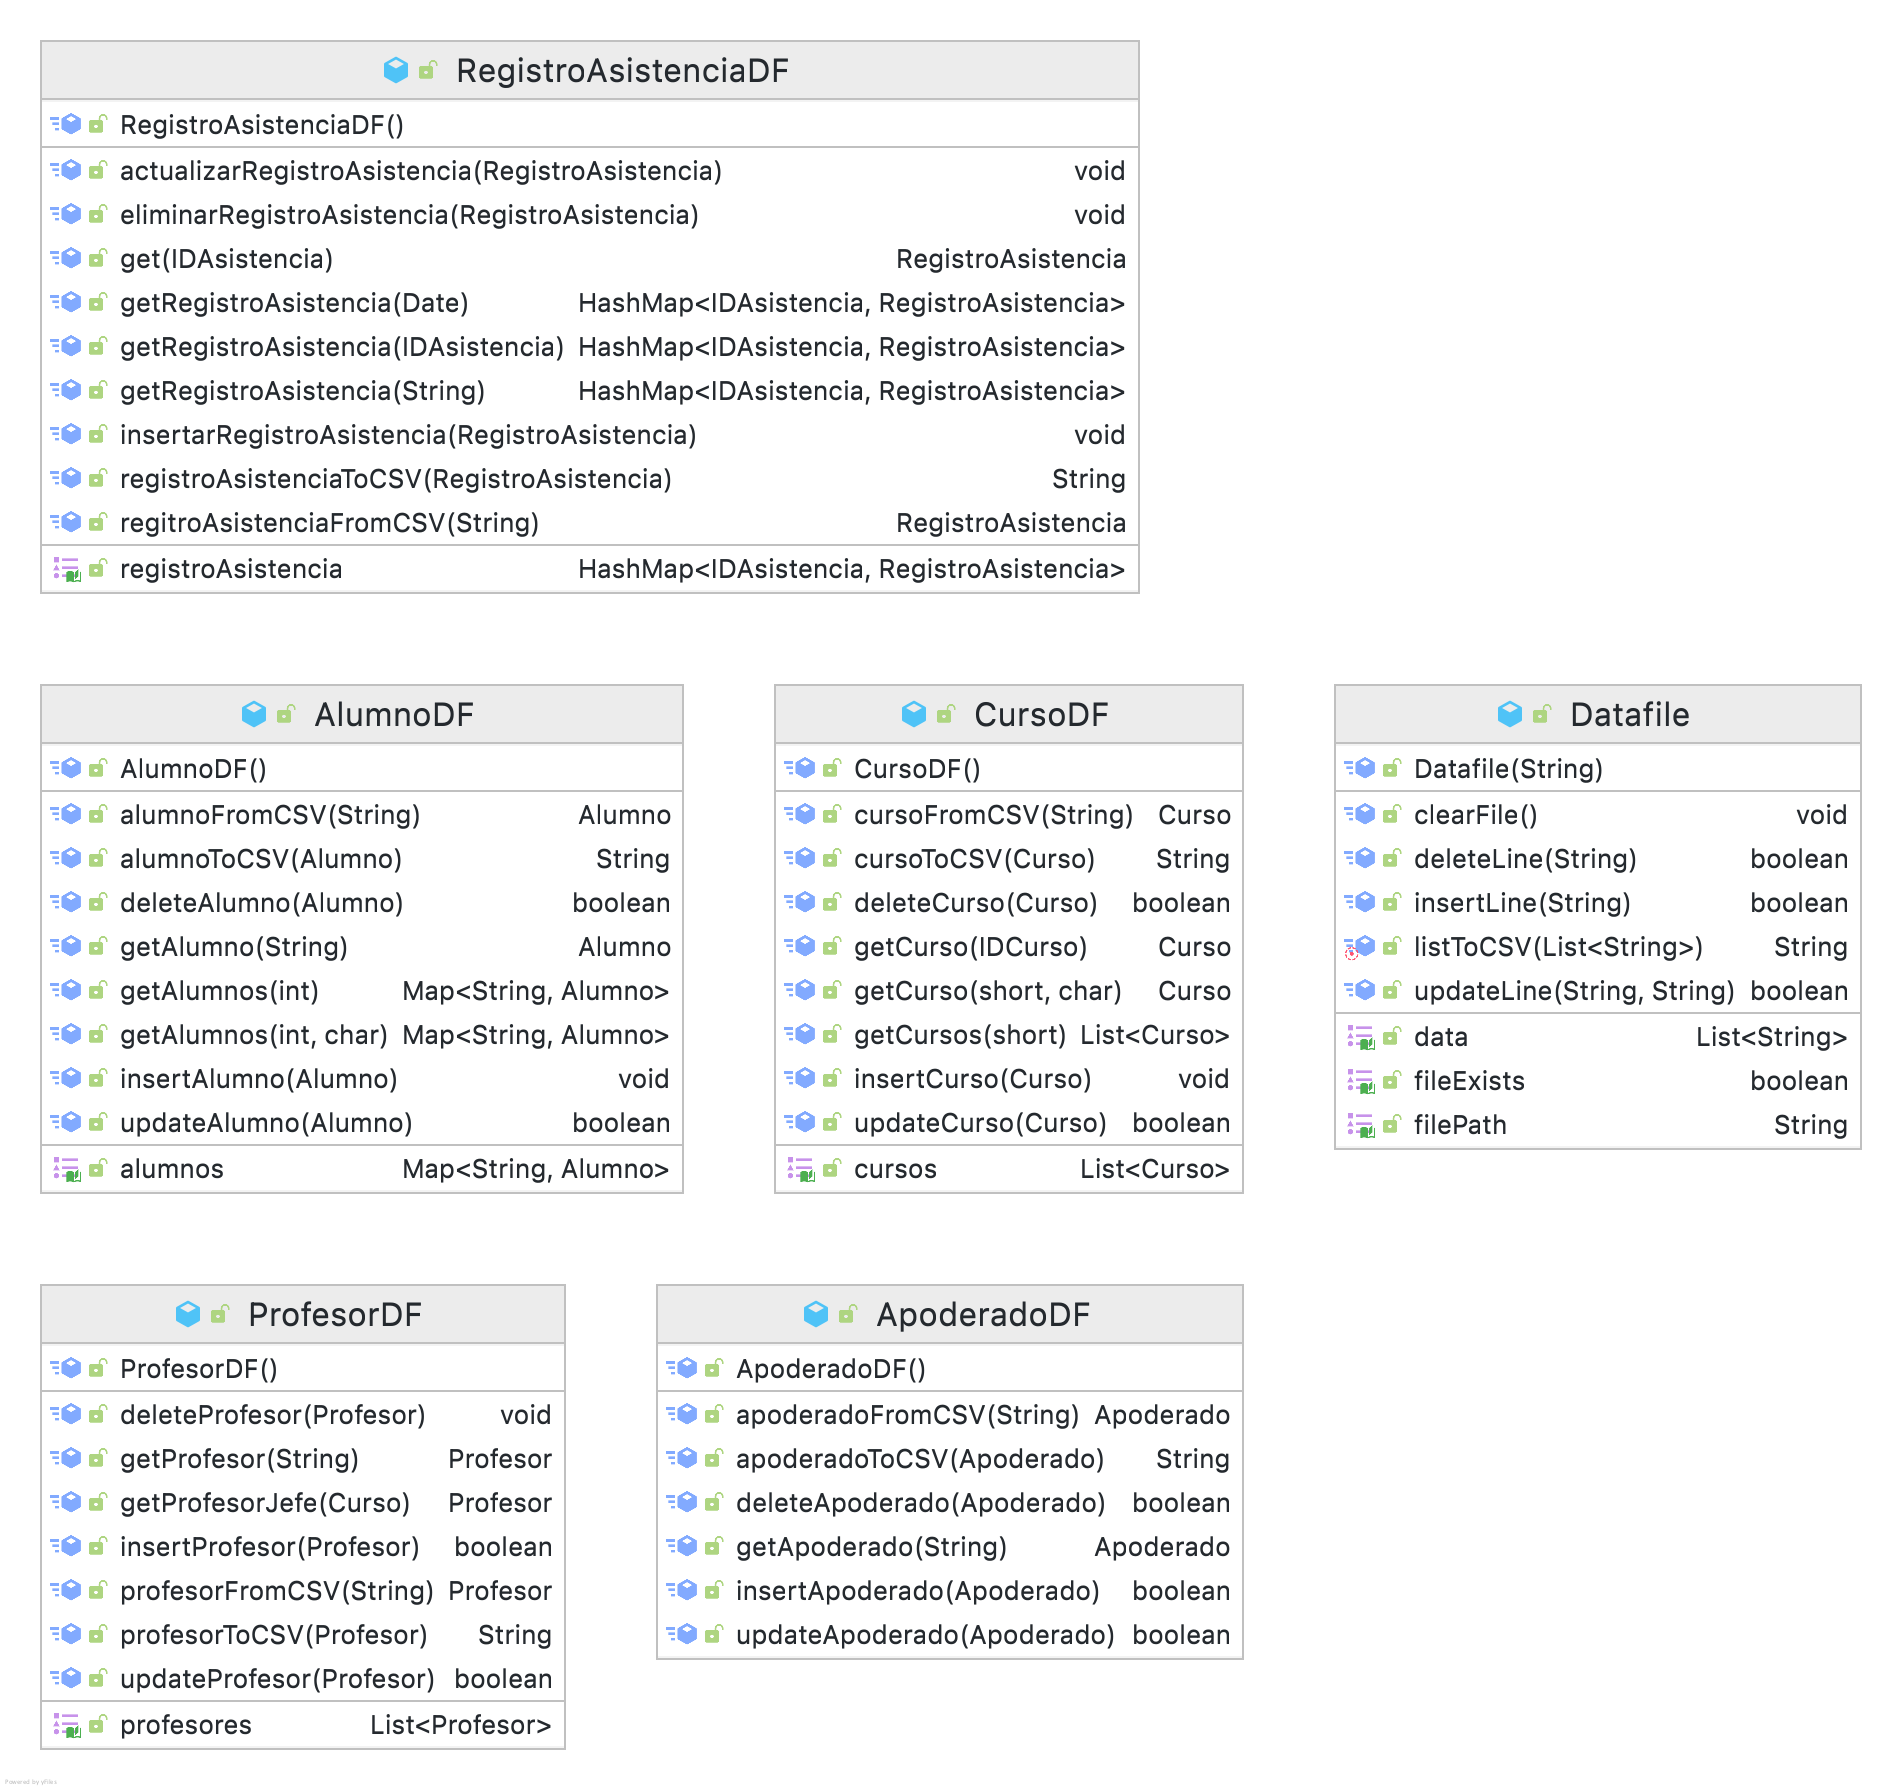
\includegraphics[width=0.9\textwidth]{contents/img/img3}
    \caption{Paquete Datafile}
    \label{fig:img3}
\end{figure}

\subsection{Todos los atributos de todas las clases deben ser privados y poseer sus respectivos métodos de lectura y escritura (getter y setter)}

Bla bla \hyperref[subsec:blablabla]{Bla}\dots

\subsection{Se deben incluir datos iniciales dentro del código}

Lorem ipsum dolor sit amet, consectetur adipiscing elit. Donec et sem luctus, finibus mauris eget, euismod arcu. Morbi at mollis risus. Praesent consequat justo tellus, ac pretium urna lacinia quis. Ut sagittis cursus finibus. Morbi pellentesque vulputate tincidunt. Aliquam at pretium tellus, et vehicula velit. Nunc turpis metus, porttitor sit amet aliquam ut, venenatis quis elit. Nam tincidunt venenatis tortor, ac sodales libero varius nec. Donec vestibulum leo a metus rutrum, vitae elementum diam suscipit. Quisque non mauris rutrum, lacinia lectus id, viverra dui. In leo quam, ultrices vitae suscipit quis, porttitor quis turpis. Vestibulum semper ligula sit amet diam scelerisque gravida.

\subsection*{Opcional: Leer datos desde archivo/base de datos}
\addcontentsline{toc}{subsection}{Opcional: Leer datos desde archivo/base de datos}

Lorem ipsum dolor sit amet, consectetur adipiscing elit. Donec et sem luctus, finibus mauris eget, euismod arcu. Morbi at mollis risus. Praesent consequat justo tellus, ac pretium urna lacinia quis. Ut sagittis cursus finibus. Morbi pellentesque vulputate tincidunt. Aliquam at pretium tellus, et vehicula velit. Nunc turpis metus, porttitor sit amet aliquam ut, venenatis quis elit. Nam tincidunt venenatis tortor, ac sodales libero varius nec. Donec vestibulum leo a metus rutrum, vitae elementum diam suscipit. Quisque non mauris rutrum, lacinia lectus id, viverra dui. In leo quam, ultrices vitae suscipit quis, porttitor quis turpis. Vestibulum semper ligula sit amet diam scelerisque gravida.
